% Created by tikzDevice version 0.10.1 on 2017-09-14 15:08:29
% !TEX encoding = UTF-8 Unicode
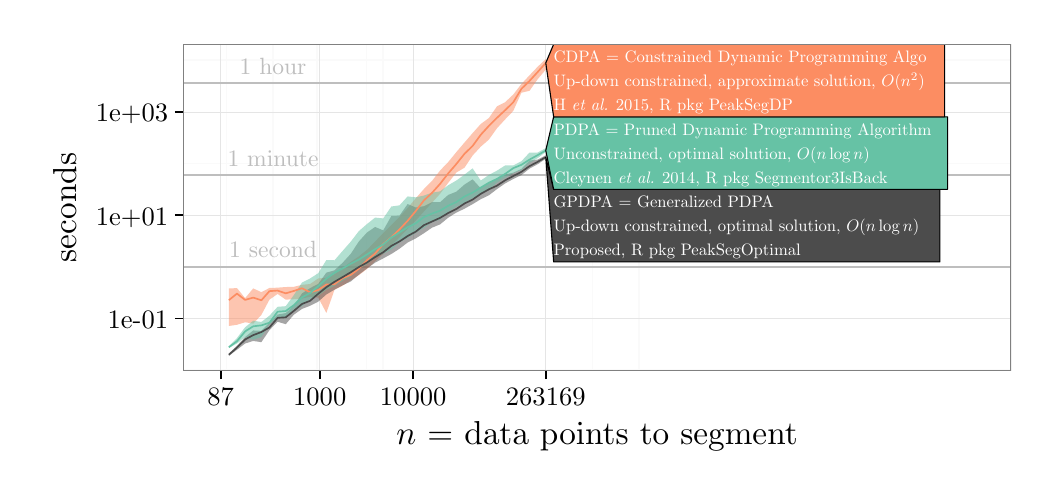
\begin{tikzpicture}[x=1pt,y=1pt]
\definecolor{fillColor}{RGB}{255,255,255}
\path[use as bounding box,fill=fillColor,fill opacity=0.00] (0,0) rectangle (361.35,158.99);
\begin{scope}
\path[clip] (  0.00,  0.00) rectangle (361.35,158.99);
\definecolor{drawColor}{RGB}{255,255,255}
\definecolor{fillColor}{RGB}{255,255,255}

\path[draw=drawColor,line width= 0.6pt,line join=round,line cap=round,fill=fillColor] (  0.00,  0.00) rectangle (361.35,158.99);
\end{scope}
\begin{scope}
\path[clip] ( 56.16, 35.02) rectangle (355.35,152.99);
\definecolor{fillColor}{RGB}{255,255,255}

\path[fill=fillColor] ( 56.16, 35.02) rectangle (355.35,152.99);
\definecolor{drawColor}{gray}{0.98}

\path[draw=drawColor,line width= 0.6pt,line join=round] ( 56.16, 35.18) --
	(355.35, 35.18);

\path[draw=drawColor,line width= 0.6pt,line join=round] ( 56.16, 72.54) --
	(355.35, 72.54);

\path[draw=drawColor,line width= 0.6pt,line join=round] ( 56.16,109.90) --
	(355.35,109.90);

\path[draw=drawColor,line width= 0.6pt,line join=round] ( 56.16,147.26) --
	(355.35,147.26);

\path[draw=drawColor,line width= 0.6pt,line join=round] ( 71.80, 35.02) --
	( 71.80,152.99);

\path[draw=drawColor,line width= 0.6pt,line join=round] ( 88.67, 35.02) --
	( 88.67,152.99);

\path[draw=drawColor,line width= 0.6pt,line join=round] (122.41, 35.02) --
	(122.41,152.99);

\path[draw=drawColor,line width= 0.6pt,line join=round] (104.52, 35.02) --
	(104.52,152.99);

\path[draw=drawColor,line width= 0.6pt,line join=round] (128.48, 35.02) --
	(128.48,152.99);

\path[draw=drawColor,line width= 0.6pt,line join=round] (204.08, 35.02) --
	(204.08,152.99);

\path[draw=drawColor,line width= 0.6pt,line join=round] (220.95, 35.02) --
	(220.95,152.99);
\definecolor{drawColor}{gray}{0.90}

\path[draw=drawColor,line width= 0.2pt,line join=round] ( 56.16, 53.86) --
	(355.35, 53.86);

\path[draw=drawColor,line width= 0.2pt,line join=round] ( 56.16, 91.22) --
	(355.35, 91.22);

\path[draw=drawColor,line width= 0.2pt,line join=round] ( 56.16,128.58) --
	(355.35,128.58);

\path[draw=drawColor,line width= 0.2pt,line join=round] (105.54, 35.02) --
	(105.54,152.99);

\path[draw=drawColor,line width= 0.2pt,line join=round] (139.29, 35.02) --
	(139.29,152.99);

\path[draw=drawColor,line width= 0.2pt,line join=round] ( 69.76, 35.02) --
	( 69.76,152.99);

\path[draw=drawColor,line width= 0.2pt,line join=round] (187.21, 35.02) --
	(187.21,152.99);
\definecolor{drawColor}{RGB}{190,190,190}

\path[draw=drawColor,line width= 0.6pt,line join=round] ( 56.16, 72.54) -- (355.35, 72.54);

\path[draw=drawColor,line width= 0.6pt,line join=round] ( 56.16,105.76) -- (355.35,105.76);

\path[draw=drawColor,line width= 0.6pt,line join=round] ( 56.16,138.97) -- (355.35,138.97);
\definecolor{fillColor}{RGB}{252,141,98}

\path[fill=fillColor,fill opacity=0.50] ( 72.69, 64.75) --
	( 75.63, 64.88) --
	( 78.57, 61.26) --
	( 81.50, 64.77) --
	( 84.44, 63.42) --
	( 87.37, 64.92) --
	( 90.31, 65.04) --
	( 93.25, 65.27) --
	( 96.18, 65.35) --
	( 99.12, 66.06) --
	(102.06, 66.36) --
	(104.99, 68.37) --
	(107.93, 68.61) --
	(110.87, 69.89) --
	(113.80, 72.07) --
	(116.74, 74.38) --
	(119.67, 76.35) --
	(122.61, 78.71) --
	(125.55, 81.73) --
	(128.48, 84.79) --
	(131.42, 87.64) --
	(134.36, 90.64) --
	(137.29, 93.80) --
	(140.23, 97.33) --
	(143.17,100.67) --
	(146.10,103.62) --
	(149.04,107.39) --
	(151.97,110.44) --
	(154.91,114.04) --
	(157.85,117.49) --
	(160.78,120.89) --
	(163.72,124.18) --
	(166.66,126.34) --
	(169.59,130.56) --
	(172.53,132.06) --
	(175.47,134.83) --
	(178.40,138.63) --
	(181.34,141.77) --
	(184.27,144.86) --
	(187.21,147.63) --
	(187.21,143.83) --
	(184.27,140.35) --
	(181.34,136.18) --
	(178.40,135.48) --
	(175.47,128.91) --
	(172.53,125.85) --
	(169.59,122.66) --
	(166.66,118.55) --
	(163.72,115.99) --
	(160.78,112.81) --
	(157.85,108.39) --
	(154.91,106.66) --
	(151.97,102.93) --
	(149.04, 98.99) --
	(146.10, 95.75) --
	(143.17, 92.53) --
	(140.23, 89.28) --
	(137.29, 86.25) --
	(134.36, 83.24) --
	(131.42, 80.34) --
	(128.48, 77.26) --
	(125.55, 74.54) --
	(122.61, 71.80) --
	(119.67, 69.55) --
	(116.74, 67.69) --
	(113.80, 65.75) --
	(110.87, 64.25) --
	(107.93, 55.92) --
	(104.99, 61.45) --
	(102.06, 61.77) --
	( 99.12, 61.10) --
	( 96.18, 60.86) --
	( 93.25, 60.72) --
	( 90.31, 62.77) --
	( 87.37, 60.72) --
	( 84.44, 55.20) --
	( 81.50, 52.05) --
	( 78.57, 52.54) --
	( 75.63, 51.63) --
	( 72.69, 51.19) --
	cycle;
\definecolor{fillColor}{RGB}{77,77,77}

\path[fill=fillColor,fill opacity=0.50] ( 72.69, 41.20) --
	( 75.63, 44.09) --
	( 78.57, 47.20) --
	( 81.50, 49.58) --
	( 84.44, 49.44) --
	( 87.37, 52.35) --
	( 90.31, 55.34) --
	( 93.25, 55.86) --
	( 96.18, 58.49) --
	( 99.12, 62.96) --
	(102.06, 64.88) --
	(104.99, 66.41) --
	(107.93, 70.47) --
	(110.87, 71.30) --
	(113.80, 74.04) --
	(116.74, 77.26) --
	(119.67, 81.73) --
	(122.61, 84.98) --
	(125.55, 86.97) --
	(128.48, 85.74) --
	(131.42, 90.94) --
	(134.36, 91.07) --
	(137.29, 95.25) --
	(140.23, 94.02) --
	(143.17, 94.48) --
	(146.10, 95.92) --
	(149.04, 95.94) --
	(151.97, 98.56) --
	(154.91, 99.73) --
	(157.85,102.31) --
	(160.78,104.17) --
	(163.72,100.94) --
	(166.66,102.79) --
	(169.59,104.47) --
	(172.53,105.95) --
	(175.47,106.60) --
	(178.40,107.96) --
	(181.34,110.98) --
	(184.27,111.34) --
	(187.21,112.86) --
	(187.21,111.62) --
	(184.27,109.63) --
	(181.34,108.05) --
	(178.40,105.71) --
	(175.47,104.31) --
	(172.53,102.71) --
	(169.59,100.66) --
	(166.66, 98.42) --
	(163.72, 97.00) --
	(160.78, 95.21) --
	(157.85, 93.58) --
	(154.91, 92.18) --
	(151.97, 90.33) --
	(149.04, 87.91) --
	(146.10, 86.72) --
	(143.17, 84.69) --
	(140.23, 82.85) --
	(137.29, 81.34) --
	(134.36, 79.11) --
	(131.42, 77.21) --
	(128.48, 75.62) --
	(125.55, 74.09) --
	(122.61, 71.98) --
	(119.67, 69.73) --
	(116.74, 67.28) --
	(113.80, 65.90) --
	(110.87, 64.32) --
	(107.93, 62.58) --
	(104.99, 59.99) --
	(102.06, 58.49) --
	( 99.12, 57.36) --
	( 96.18, 55.27) --
	( 93.25, 51.84) --
	( 90.31, 52.73) --
	( 87.37, 49.71) --
	( 84.44, 45.34) --
	( 81.50, 45.79) --
	( 78.57, 44.86) --
	( 75.63, 42.61) --
	( 72.69, 40.39) --
	cycle;
\definecolor{fillColor}{RGB}{102,194,165}

\path[fill=fillColor,fill opacity=0.50] ( 72.69, 43.82) --
	( 75.63, 46.82) --
	( 78.57, 50.73) --
	( 81.50, 53.09) --
	( 84.44, 52.64) --
	( 87.37, 54.92) --
	( 90.31, 58.12) --
	( 93.25, 58.35) --
	( 96.18, 62.36) --
	( 99.12, 66.88) --
	(102.06, 68.37) --
	(104.99, 70.27) --
	(107.93, 75.02) --
	(110.87, 74.94) --
	(113.80, 78.32) --
	(116.74, 81.66) --
	(119.67, 85.48) --
	(122.61, 88.03) --
	(125.55, 90.36) --
	(128.48, 90.06) --
	(131.42, 94.37) --
	(134.36, 94.79) --
	(137.29, 98.01) --
	(140.23, 97.69) --
	(143.17, 98.32) --
	(146.10, 99.35) --
	(149.04, 99.85) --
	(151.97,102.05) --
	(154.91,103.76) --
	(157.85,105.89) --
	(160.78,108.16) --
	(163.72,103.76) --
	(166.66,105.78) --
	(169.59,107.34) --
	(172.53,109.20) --
	(175.47,109.22) --
	(178.40,110.71) --
	(181.34,113.86) --
	(184.27,113.88) --
	(187.21,115.46) --
	(187.21,114.10) --
	(184.27,111.82) --
	(181.34,110.11) --
	(178.40,107.54) --
	(175.47,106.44) --
	(172.53,104.78) --
	(169.59,103.02) --
	(166.66,100.45) --
	(163.72, 98.81) --
	(160.78, 97.42) --
	(157.85, 95.64) --
	(154.91, 94.34) --
	(151.97, 92.35) --
	(149.04, 89.68) --
	(146.10, 88.73) --
	(143.17, 86.64) --
	(140.23, 84.88) --
	(137.29, 83.01) --
	(134.36, 81.41) --
	(131.42, 78.81) --
	(128.48, 77.31) --
	(125.55, 76.02) --
	(122.61, 73.52) --
	(119.67, 71.88) --
	(116.74, 69.11) --
	(113.80, 67.51) --
	(110.87, 65.69) --
	(107.93, 64.30) --
	(104.99, 62.10) --
	(102.06, 61.00) --
	( 99.12, 58.35) --
	( 96.18, 57.36) --
	( 93.25, 54.02) --
	( 90.31, 54.10) --
	( 87.37, 51.84) --
	( 84.44, 47.20) --
	( 81.50, 46.22) --
	( 78.57, 47.20) --
	( 75.63, 44.86) --
	( 72.69, 43.24) --
	cycle;
\definecolor{drawColor}{RGB}{252,141,98}

\path[draw=drawColor,line width= 0.6pt,line join=round] ( 72.69, 60.53) --
	( 75.63, 62.89) --
	( 78.57, 60.62) --
	( 81.50, 61.45) --
	( 84.44, 60.47) --
	( 87.37, 63.79) --
	( 90.31, 63.99) --
	( 93.25, 62.99) --
	( 96.18, 63.86) --
	( 99.12, 64.82) --
	(102.06, 63.36) --
	(104.99, 64.18) --
	(107.93, 66.19) --
	(110.87, 66.28) --
	(113.80, 68.46) --
	(116.74, 69.66) --
	(119.67, 71.88) --
	(122.61, 74.98) --
	(125.55, 77.38) --
	(128.48, 80.83) --
	(131.42, 83.28) --
	(134.36, 86.10) --
	(137.29, 89.19) --
	(140.23, 92.74) --
	(143.17, 96.57) --
	(146.10, 99.29) --
	(149.04,102.58) --
	(151.97,106.34) --
	(154.91,109.75) --
	(157.85,113.42) --
	(160.78,116.26) --
	(163.72,120.29) --
	(166.66,123.51) --
	(169.59,126.42) --
	(172.53,129.17) --
	(175.47,132.04) --
	(178.40,136.86) --
	(181.34,139.75) --
	(184.27,142.95) --
	(187.21,146.24);
\definecolor{drawColor}{gray}{0.30}

\path[draw=drawColor,line width= 0.6pt,line join=round] ( 72.69, 40.80) --
	( 75.63, 43.39) --
	( 78.57, 46.32) --
	( 81.50, 47.90) --
	( 84.44, 49.01) --
	( 87.37, 50.67) --
	( 90.31, 54.14) --
	( 93.25, 54.33) --
	( 96.18, 56.65) --
	( 99.12, 59.15) --
	(102.06, 60.29) --
	(104.99, 62.84) --
	(107.93, 65.19) --
	(110.87, 67.16) --
	(113.80, 68.86) --
	(116.74, 70.60) --
	(119.67, 72.49) --
	(122.61, 74.13) --
	(125.55, 76.10) --
	(128.48, 77.84) --
	(131.42, 80.13) --
	(134.36, 81.75) --
	(137.29, 83.70) --
	(140.23, 85.28) --
	(143.17, 87.61) --
	(146.10, 88.94) --
	(149.04, 90.27) --
	(151.97, 92.02) --
	(154.91, 93.47) --
	(157.85, 95.45) --
	(160.78, 96.87) --
	(163.72, 98.94) --
	(166.66,100.57) --
	(169.59,101.91) --
	(172.53,103.85) --
	(175.47,105.37) --
	(178.40,106.89) --
	(181.34,108.96) --
	(184.27,110.50) --
	(187.21,112.23);
\definecolor{drawColor}{RGB}{102,194,165}

\path[draw=drawColor,line width= 0.6pt,line join=round] ( 72.69, 43.53) --
	( 75.63, 45.68) --
	( 78.57, 49.23) --
	( 81.50, 51.08) --
	( 84.44, 51.42) --
	( 87.37, 52.40) --
	( 90.31, 56.35) --
	( 93.25, 56.59) --
	( 96.18, 58.72) --
	( 99.12, 61.52) --
	(102.06, 63.13) --
	(104.99, 65.59) --
	(107.93, 68.29) --
	(110.87, 70.41) --
	(113.80, 71.97) --
	(116.74, 73.69) --
	(119.67, 75.18) --
	(122.61, 77.05) --
	(125.55, 78.96) --
	(128.48, 80.67) --
	(131.42, 83.16) --
	(134.36, 85.02) --
	(137.29, 86.88) --
	(140.23, 88.29) --
	(143.17, 90.54) --
	(146.10, 91.81) --
	(149.04, 92.87) --
	(151.97, 94.66) --
	(154.91, 95.97) --
	(157.85, 98.01) --
	(160.78, 99.40) --
	(163.72,101.20) --
	(166.66,102.97) --
	(169.59,104.35) --
	(172.53,106.15) --
	(175.47,108.23) --
	(178.40,109.43) --
	(181.34,111.32) --
	(184.27,112.92) --
	(187.21,114.61);
\definecolor{drawColor}{RGB}{190,190,190}

\node[text=drawColor,anchor=base,inner sep=0pt, outer sep=0pt, scale=  0.85] at ( 88.67, 75.78) {1 second};

\node[text=drawColor,anchor=base,inner sep=0pt, outer sep=0pt, scale=  0.85] at ( 88.67,109.00) {1 minute};

\node[text=drawColor,anchor=base,inner sep=0pt, outer sep=0pt, scale=  0.85] at ( 88.67,142.22) {1 hour};
\end{scope}
\begin{scope}
\path[clip] ( 56.16, 35.02) rectangle (355.35,152.99);
\definecolor{drawColor}{RGB}{0,0,0}
\definecolor{fillColor}{gray}{0.30}

\path[draw=drawColor,line width= 0.4pt,line join=round,line cap=round,fill=fillColor] (187.21,112.23) --
	(190.06,100.57) --
	(329.63,100.57) --
	(329.63, 74.36) --
	(190.06, 74.36) --
	cycle;
\definecolor{fillColor}{RGB}{102,194,165}

\path[draw=drawColor,line width= 0.4pt,line join=round,line cap=round,fill=fillColor] (187.21,114.61) --
	(190.06,126.78) --
	(332.41,126.78) --
	(332.41,100.57) --
	(190.06,100.57) --
	cycle;
\definecolor{fillColor}{RGB}{252,141,98}

\path[draw=drawColor,line width= 0.4pt,line join=round,line cap=round,fill=fillColor] (187.21,146.24) --
	(190.06,152.99) --
	(331.33,152.99) --
	(331.33,126.78) --
	(190.06,126.78) --
	cycle;
\definecolor{drawColor}{RGB}{255,255,255}

\node[text=drawColor,anchor=base west,inner sep=0pt, outer sep=0pt, scale=  0.60] at (190.06, 93.83) {GPDPA = Generalized PDPA};

\node[text=drawColor,anchor=base west,inner sep=0pt, outer sep=0pt, scale=  0.60] at (190.06, 85.19) {Up-down constrained, optimal solution, $O(n \log n)$};

\node[text=drawColor,anchor=base west,inner sep=0pt, outer sep=0pt, scale=  0.60] at (190.06, 76.55) {Proposed, R pkg PeakSegOptimal};

\node[text=drawColor,anchor=base west,inner sep=0pt, outer sep=0pt, scale=  0.60] at (190.06,120.04) {PDPA = Pruned Dynamic Programming Algorithm};

\node[text=drawColor,anchor=base west,inner sep=0pt, outer sep=0pt, scale=  0.60] at (190.06,111.40) {Unconstrained, optimal solution, $O(n \log n)$};

\node[text=drawColor,anchor=base west,inner sep=0pt, outer sep=0pt, scale=  0.60] at (190.06,102.76) {Cleynen {\it et al.} 2014, R pkg Segmentor3IsBack};

\node[text=drawColor,anchor=base west,inner sep=0pt, outer sep=0pt, scale=  0.60] at (190.06,146.25) {CDPA = Constrained Dynamic Programming Algo};

\node[text=drawColor,anchor=base west,inner sep=0pt, outer sep=0pt, scale=  0.60] at (190.06,137.61) {Up-down constrained, approximate solution, $O(n^2)$};

\node[text=drawColor,anchor=base west,inner sep=0pt, outer sep=0pt, scale=  0.60] at (190.06,128.97) {H {\it et al.} 2015, R pkg PeakSegDP};
\definecolor{drawColor}{gray}{0.50}

\path[draw=drawColor,line width= 0.6pt,line join=round,line cap=round] ( 56.16, 35.02) rectangle (355.35,152.99);
\end{scope}
\begin{scope}
\path[clip] (  0.00,  0.00) rectangle (361.35,158.99);
\definecolor{drawColor}{RGB}{0,0,0}

\node[text=drawColor,anchor=base east,inner sep=0pt, outer sep=0pt, scale=  0.96] at ( 50.76, 50.21) {1e-01};

\node[text=drawColor,anchor=base east,inner sep=0pt, outer sep=0pt, scale=  0.96] at ( 50.76, 87.57) {1e+01};

\node[text=drawColor,anchor=base east,inner sep=0pt, outer sep=0pt, scale=  0.96] at ( 50.76,124.93) {1e+03};
\end{scope}
\begin{scope}
\path[clip] (  0.00,  0.00) rectangle (361.35,158.99);
\definecolor{drawColor}{RGB}{0,0,0}

\path[draw=drawColor,line width= 0.6pt,line join=round] ( 53.16, 53.86) --
	( 56.16, 53.86);

\path[draw=drawColor,line width= 0.6pt,line join=round] ( 53.16, 91.22) --
	( 56.16, 91.22);

\path[draw=drawColor,line width= 0.6pt,line join=round] ( 53.16,128.58) --
	( 56.16,128.58);
\end{scope}
\begin{scope}
\path[clip] (  0.00,  0.00) rectangle (361.35,158.99);
\definecolor{drawColor}{RGB}{0,0,0}

\path[draw=drawColor,line width= 0.6pt,line join=round] (105.54, 32.02) --
	(105.54, 35.02);

\path[draw=drawColor,line width= 0.6pt,line join=round] (139.29, 32.02) --
	(139.29, 35.02);

\path[draw=drawColor,line width= 0.6pt,line join=round] ( 69.76, 32.02) --
	( 69.76, 35.02);

\path[draw=drawColor,line width= 0.6pt,line join=round] (187.21, 32.02) --
	(187.21, 35.02);
\end{scope}
\begin{scope}
\path[clip] (  0.00,  0.00) rectangle (361.35,158.99);
\definecolor{drawColor}{RGB}{0,0,0}

\node[text=drawColor,anchor=base,inner sep=0pt, outer sep=0pt, scale=  0.96] at (105.54, 22.32) {1000};

\node[text=drawColor,anchor=base,inner sep=0pt, outer sep=0pt, scale=  0.96] at (139.29, 22.32) {10000};

\node[text=drawColor,anchor=base,inner sep=0pt, outer sep=0pt, scale=  0.96] at ( 69.76, 22.32) {87};

\node[text=drawColor,anchor=base,inner sep=0pt, outer sep=0pt, scale=  0.96] at (187.21, 22.32) {263169};
\end{scope}
\begin{scope}
\path[clip] (  0.00,  0.00) rectangle (361.35,158.99);
\definecolor{drawColor}{RGB}{0,0,0}

\node[text=drawColor,anchor=base,inner sep=0pt, outer sep=0pt, scale=  1.20] at (205.75,  8.40) {$n$ = data points to segment};
\end{scope}
\begin{scope}
\path[clip] (  0.00,  0.00) rectangle (361.35,158.99);
\definecolor{drawColor}{RGB}{0,0,0}

\node[text=drawColor,rotate= 90.00,anchor=base,inner sep=0pt, outer sep=0pt, scale=  1.20] at ( 17.52, 94.01) {seconds};
\end{scope}
\end{tikzpicture}
